\chapter{Cyfrowy system wizyjny}
\label{cha:csw}

\section{Podczerwień}

Jako podczerwień określa się promieniowanie elektromagnetyczne w zakresie długości fali od  0,75 $\mu m$ do 1000~$\mu m$. Ciało które ma temperaturę powyżej zera absolutnego emituje swoją powierzchnią promieniowanie. Im większa jest temperatura ciała tym większa jest jego emisja. Dla każdej temperatury danego ciała istnieje charakterystyczna długość fali o najwyższej wartości mocy promieniowania. Im wyższa temperatura tym ta częstotliwość przesuwa się w zakres fal widzialnych. Można to zaobserwować gdy stal osiąga wysoką temperaturę powodując tym emisję światła. Ciało doskonale czarne całkowicie pochłania padające na nie promieniowanie, oraz emituję promieniowanie ściśle związane z jego temperaturą. Wykres na rysunku \ref{fig:perfect_black}  przedstawia tą charakterystykę. Promieniowanie podczerwone jest częściowo pochłaniane przez atmosferę ziemską . Na rysunku  \ref{fig:atmosfera_int} przedstawiono transmisyjność atmosfery. W aparaturze obrazującej w podczerwieni wykorzystuję się dwa zakresy przy których transmisyjność jest największa:  3 -- 5 $\mu m$ (MIWR, ang. \textit{mid wave infrared} - podczerwień fal średnich) oraz  8 -- 14 $\mu m$ (LWIR , ang. \textit{long wave infrared} - podczeriwń fal długich)\cite{niklaus2007mems}.

\begin{figure}
\centering
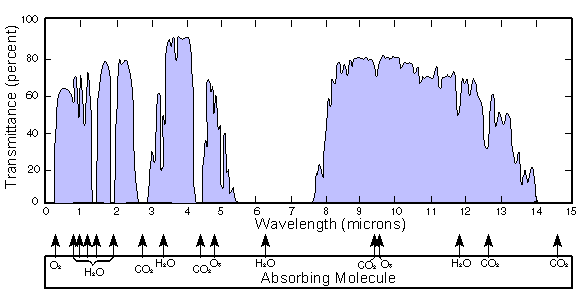
\includegraphics[width=0.8\linewidth]{images/Atmosfaerisk_spredning}
\caption[Wykres transmisyjności atmosfery dla promieniowania podczerwonego ]{Wykres transmisyjności atmosfery dla promieniowania podczerwonego \cite{wiki:infrared}.}
\label{fig:perfect_black}
\end{figure}

\begin{figure}
\centering
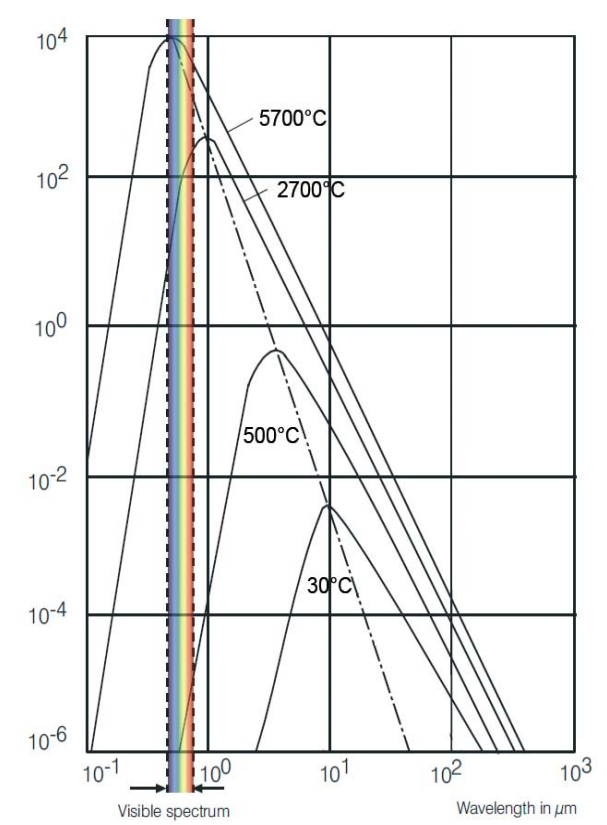
\includegraphics[width=0.4\linewidth]{images/perfect_black_emi}
\caption[Emisyjność ciała idealnie czarnego]{Emisyjność ciała idealnie czarnego.}
\label{fig:atmosfera_int}
\end{figure}

\section{Metody akwizycja obrazu}

Większość implementacji wykorzystuje układ dwóch równoległych do siebie kamer. Do połączenia obrazów należy zastosować algorytm wyrównujący oba obrazy. Kalibrację wykonuję się specjalnymi  planszami które pozwalają określić położenie punktów kalibracyjnych w obu rejestrowanych zakresach. Plansze mogą być aktywne (posiadają własne źródło ciepła) albo pasywne (przesłaniają obce źródło ciepła). W tym układzie występuję również zjawisko paralaksy które powiększa się wraz z wzrostem odległości obiektu od punktu kalibracji. W pracy  \cite{hwang2015multispectral} autorzy zastosowali zwierciadło półprzezroczyste wykonane z wafla krzemowego pokrytego cynkiem do rozdzielenia obrazu co wyeliminowało wady układu równoległego.

\begin{figure}[h]
	\centering
	\begin{subfigure}{0.45\textwidth}
		\centering
		 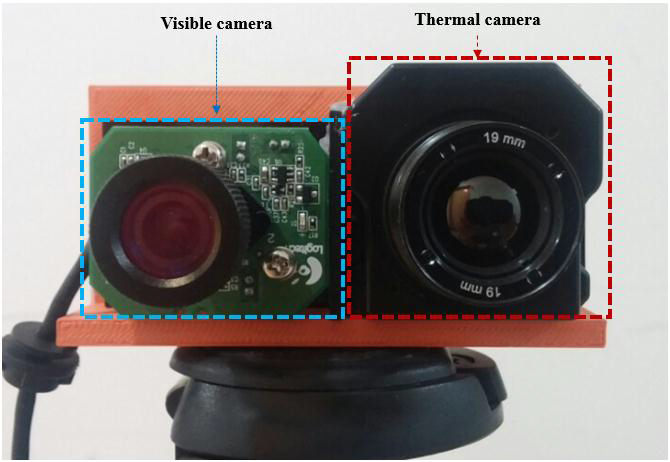
\includegraphics[width=1\textwidth]{images/dual-camera}
		\subcaption{\label{dual_camera}}
	\end{subfigure}
	\begin{subfigure}{0.45\textwidth}
		\centering
		 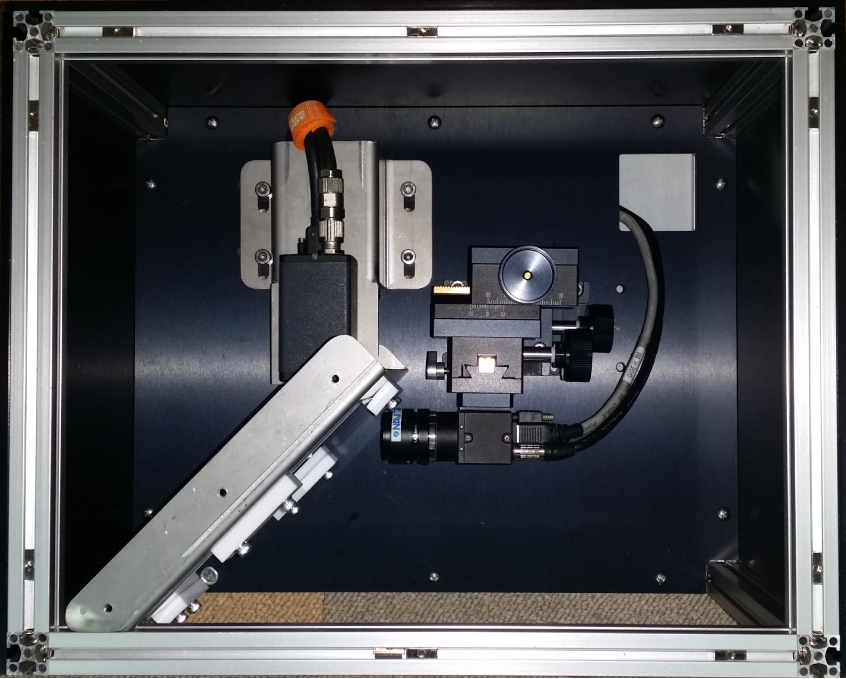
\includegraphics[width=1\textwidth]{images/multispectral}
		\subcaption{\label{multispectral}}
	\end{subfigure}
	
	\caption{\label{fig:cameras_systems}Sposoby akwizycji obrazów:  \protect\subref{dual_camera} dwie kamery równolegle \cite{lee2015robust}, \protect\subref{multispectral} z wykorzystaniem zwierciadła półprzezroczystego \cite{hwang2015multispectral}.}
\end{figure}

\section{Model geometryczny}

Do opisu matematycznego systemu wykorzystuje się model kamery otworowej. Dzięki niej można opisać relację między trójwymiarową przestrzenią a dwuwymiarowym obrazem za pomocą projekcji perspektywicznych. Nie stanowi on najdokładniejszego opisu matematycznego kamery, nie ma uwzględnionych w nim zakłóceń soczewkowych, ale jest wystarczające dobre dla niektórych zastosowań. Składa się ona z 2 zestawów parametrów: zewnętrznych oraz wewnętrznych. Parametry zewnętrzne definiują lokację kamery względem zewnętrznego układu współrzędnych. Są reprezentowane przez wektor translacji \(T\) między układem związanym z kamerą \( \left (  X_{c},Y_{c},Z_{c}\right ) \)
 a zewnętrznym \(\left (  X,Y,Z\right )\). Drugim parametrem jest macierz rotacji \( R \)( między osiami tych dwóch układów.
Punkt \(P = \left [ X,Y,Z \right ]^T \) będący w zewnętrznym układzie współrzędnym ma swój odpowiednik w układzie wewnętrznym który można określić zależnością 

\begin{equation}
P_{c} = RP+T
\end{equation}

Właściwości optyczne kamery można przedstawić w postaci macierzy kamery.

\begin{equation}
K = \begin{bmatrix}
f_x & 0 & x_0 \\ 
0 & f_y & y_0\\ 
0 &0  & 1
\end{bmatrix}
\end{equation}
gdzie:
\begin{conditions}
f_{x}, f_{y} & ogniskowa kamery wyrażona w liczbie pikseli, \\
x_{0},y_{0} & współrzęne punktu głównego. 
\end{conditions}

Macierz K określa związek między między znormalizowanymi współrzędnymi w układzie odniesienia kamery, danych wzorem \(x_n = \frac{X_c}{Z_c}, y_n = \frac{Y_c}{Z_c}\), a odpowiadającym im wspórzędnymi punktów na obrazie \(u,v\):

\begin{equation}
\begin{bmatrix}
u \\
v \\
1
\end{bmatrix} = K \begin{bmatrix}
x_n \\
y_n \\
1
\end{bmatrix}
\end{equation}



\section{Algorytmy detekcji pieszych}

W cyfrowej analizie obrazu rozpoznawanie pieszych jest jedną z najbardziej aktywnych i rozwijanych dziedzin. W przeciągu kilkudziesięciu lat powstało ponad tysiąc artykułów poruszających to zagadnienie \cite{zhang2015filtered} i wiele różnych metod zostało już opracowanych. Większość metod opiera się o analizę obrazu tylko w jednym spektrum: widzialnym albo podczerwieni. Praca \cite{hwang2015multispectral} pokazała że połączenie obu obrazów może dać lepsze wyniki. Podobnie w \cite{gonzalez2016pedestrian} ustalono że analiza multispektralna jest skuteczniejsza w dzień niż w nocy (o około 5\% AMR (ang. avrange miss rate).   W artykule \cite{benenson2014ten} autorzy podsumowują osiągnięcia w dziedzinie detekcji pieszych w latach 2004 – 2014 wyróżniono ponad 40 różnych podejść do problemu. Artykuł jest oparty o bazę danych Caltech-USA która oferuje obrazy w kolorze. Jednym z wniosków jest że przez ostanie dziesięć lat największy postęp został osiągnięty głównie dzięki dopracowaniu cech jakie są wyodrębniane z obrazu niż ulepszanie klasyfikatora. Dodatkowo autorzy połączyli cechy dające najlepsze wyniki i stworzyli własną metodę która uzyska 12\% zysk AMR względem  najlepszej badanej wcześniej metody.

Dla typowego algorytmu detekcji pieszych można wyróżnić trzy podstawowe etapy:

\subsection{Ustalenie regionu zainteresowań} 
Jest to obszar zwany ROI(ang. Region of interest) w którym potencjalnie mogą znajdować się przechodnie. Wiele podejść uznaje cały obraz jako ROI i stosuje okno przesuwne sprawdzając każdy możliwy fragment obrazu. Jeżeli obraz jest rejestrowany przez nieruchomą kamerę, ROI można określić poprzez różnicę między zapamiętanym tłem a aktualnym obrazem. Wyodrębnienie ROI jest bardzo istotne w przypadku pracy w czasie rzeczywistym ze względu na ograniczony czas analizy pojedynczego obrazu.

\subsection{Wyodrębnienie cech}

Do najbardziej popularnych cech można zaliczyć:

\begin{enumerate}
\item Histogramy zorientowanych gradientów (HOG) zaproponowany przez N.Dalala i B. Triggs w pracy \cite{dalal2005histograms} stała się jedną z najbardziej popularnych techniką w dziedzinie rozpoznawania ludzi. Jest cały czas rozwijana i modyfikowana w wielu pracach naukowych. Technika polega na zliczeniu kierunków gradientów, uzyskanych z 2 masek kierunkowych \(\begin{bmatrix}-1 & 0 & 1\end{bmatrix} \) i \( \begin{bmatrix}-1 & 0 & 1 \end{bmatrix}^T\), w komórkach o określonych wymiarach. Komórki te są organizowane w bloki w obrębie których następuję normalizacja. Wektorem cech jest połączony wszystkich histogramów z wszystkich bloków w jeden wektor.

\item Lokalne wzorce binarne LBP (ang. Local Binary Paterns).  Oryginalnie przeznaczone do opisu tekstur. Obraz zostaje podzielony na bloki. Następnie każdego piksela w bloku zostaje przypisany wzorzec binarny na podstawie wartości pikseli w jego sąsiedztwie. Jeżeli wartość sąsiadującego piksela jest większa od centralnego to przyjmuje on wartość 1. Następnie zostaje obliczony histogram dla każdego bloku. Histogramy z wszystkich bloków wchodzących w skład obrazu tworzą wektor cech \cite{ojala2002multiresolution}.

\item Falki Haara.
Określają różnicę w kontraście między dwoma przylegającymi prostokątnymi obszarami. Są łatwe do skalowania i nie wymagają dużych nakładów obliczeniowych.

\item Kolor. W analizie obrazo wykorzystuje różne przestrzenie barw np. RGB, HSV oraz LUV. 

\item Lokalne struktury. W odróżnieniu od pojedynczych pikseli można wyznaczyć lokalne struktury o podobnym kolorze. (np. głowa i ręce mają podobne kolory, jednolita koszula, spodnie)


\end{enumerate}

\subsection{Klasyfikator}
Otrzymany wektor cech jest poddany klasyfikacji której wynik decyduje czy obraz zawiera człowieka. W pracy \cite{benenson2014ten} autorzy wyróżnili 3 dominujące rodziny:

\begin{enumerate}
\item Rodzina DPM (ang. Deformable Part Detectors) ??? wykrywacze deformowlnych elementów ???. Technika polega na klasyfikacji poszczególnych elementów człowieka (głowa, tułów, nogi). Następnie  jest analizowany układ tych elementów na obrazie i podjęcie decyzji o obecności człowieka.

\item Deep networks – głębokie sieci neuronowe.

\item Decision forests – ?? lasy decyzyjne ?? zbiór nieskorelowanych drzew decyzyjnych.

\item inne: SVN (ang. support vector machine – maszyna wektorów nośnych), AdaBoost itp.
\end{enumerate}

\section{Wykorzystanie FPGA w analizie obrazu}

Tradycyjne systemy wizyjne zwykle bazują na architekturze sekwencyjnej, po kolejnym przekształceniu obraz jest sukcesywnie poddawany następnym. W aplikacji procesorowej te operacje są wykonywane przez układ arytmetyczno-logiczny w który jest wyposażony. Kolejne kroki algorytmu są kompilowane w ciąg instrukcji dla procesora który oprócz operacji matematycznych dużą część pracy poświęca na pobieranie i dekodowanie rozkazów oraz na pobieranie i zapisywanie danych do pamięci. By taka aplikacja mogła pracować w czasie rzeczywistym cała procedura musi wykonać się szybciej przychodzące dane obrazu co wymusza wysoki taktowanie procesora sięgające GHz. 

W przypadku podejścia równoległego, implementacja poszczególnych kroków algorytmu odbywa się w osobnych procesach. Jeżeli kolejne kroki algorytmu wymagałyby danych otrzymanych z poprzednich to zysk takiego zabiegu byłby równy zero.  By uzyskać znacznie przyspieszenie algorytm musi mieć możliwość podzielenia na wiele niezależnych części. Maksymalne do uzyskania przyspieszenie jest określone przez prawo Amdahla: 
\begin{equation}
P_w =\frac{1}{ s + \frac{1-s}{n_w}}
\end{equation}
gdzie:
\begin{conditions}
P_{w} &  przyspieszenie algorytmu w systemie wieloprocesorowym, \\
s &  cześć algorytmu niepodlegająca zrównolegleniu (wartość od zera do jeden), \\
n_{w} & liczba elementów obliczeniowych.
\end{conditions}

Teoretycznie jedynym ograniczaniem w możliwości zrównolegnia obliczeń jest ilość zasobów dostępnych, jednak istotnym aspektem jest sposób dostarczania danych do zaimplementowanych w układzie procesorów. Czas i przepustowość jaka jest potrzebna do odczytania i zapisu obrazu po przetworzeniu z i do pamięci jest najczęściej wąskim gardłem systemu wizyjnego. Z tego powodu przetwarzanie obrazu bezpośrednio z sensora w czasie jego akwizycji jest chętnie wykorzystywane gdyż zmniejsza to ilość operacji odczytu i zapisu.  \cite{garcia2014survey}

\section{Przegląd literatury}

\subsection{Podobne rozwiązania}

W pracy \cite{kolzpoz} autorzy opracowali algorytm pozwalający na szybką i efektywną detekcję przechodniów w czasie rzeczywistym . Termowizja pozwala na uzyskanie dobrego kontrastu między poszukiwanym przechodniem a otoczeniem. System dedykowany jest do pracy w nocy kiedy kontrast między człowiekiem pozwala na jednoznaczne ich rozróżnienie. Rozwiązanie bazuję na ulepszonym algorytmie progowania i segmentacji obrazu. Pierwszym etapem jest wyodrębnienie obszarów zainteresowań (ang. ROI). Pozwala to na znaczne ograniczenie obszaru obrazu do analizy. Obraz w odcieniach szarości zostaję poddany binaryzacji z użyciem dwóch progów: mniejszym i większym. Dodatkowo każdy wykryty obszar tworzy dodatkowy ROI przylegający do pierwotnego. Progowanie z pojedynczym progiem jest niewystarczające w wielu wypadach dlatego autorzy zastosowali podwójne progowanie. Pozwala to na detekcję przechodniów w różnych rejonach obrazu o różnym kontraście. Progi zmieniają się wraz z dynamiką obrazu wejściowego. W obrazie termicznym człowieka często występuję obszar o niższej temperaturze w okolicach bioder. Skutkuje to przerwą w zbinearyzowanym obiekcie i błędną klasyfikację np.: samych nóg. Autorzy opracowali technikę polegającą na powiększeniu obszaru. Łączy ona dwie połówki człowieka jeżeli posiadaj wspólne współrzędne wzdłuż pionowej osi tworząc nowy obszar. Ostatecznie obie grupy obszarów zainteresowania uzyskanych z obu progowań zostają połączone. 

Następnym krokiem jest filtracja wyników. Ma na celu zredukowanie ilości obszarów do końcowej analizy. Autorzy zastosowali filtrację opierającą się na proporcji obszaru zainteresowań. Pozytywnie zakwalifikowane zostały tylko obszary o odpowiednich proporcja wysokości do szerokości (1:1.3 do 1:4). Z racji że badany obraz pochodzi z kamery zamontowanej na stałe na samochodzie autorzy wykorzystali filtrację perspektywiczną. W większej odległości na horyzoncie obiekty są mniejsze. Zakłada ona że w określonych obszarach obrazu istnieje maksymalna możliwa wysokość kandydata. Filtracja jednorodnych regionów pozwoliła na odrzucenie obszarów które często występują jako część szerszych obiektów nie mających nic wspólnego z przechodnimi. Autorzy zaproponowali by obliczenie odchylenia standardowego tych obszarów w odcieniach szarości i odrzucenie części która jest poniżej pewnego progu. 

Ostatnim krokiem algorytmu jest klasyfikacja wytypowanych kandydatów. Autorzy wykorzystują Histogram zorientowanych gradientów jako cechę tworząc wektor 3780 cech które są przetwarzane przez maszynę wektorów nośnych.

W celu zbadania dokładności algorytmu został przeprowadzony test na zbiorze CVC-14 zawierający obrazy nagrane kamerą FIR podczas nocnego przejazdu samochodem. Testy wykazały że metoda podwójnego progowania daje trzy razy lepsze rezultaty niż przy wykorzystaniu pojedynczego progu. Wraz z zaproponowanymi technikami filtracji zaowocowało bardzo efektywnym mechanizmem segmentacji. Cała procedura detekcji przechodniów osiągnęła wysoki poziom wydajności na poziomie 33 klatek na sekundę przy wykorzystaniu pojedynczego rdzenia CPU.


„Pedestrian detection using infrared images and histograms of oriented gradients”

W pracy [] autorzy zaproponowali wykorzystanie dwóch kamer termowizyjnych tworząc system stereowizyjny. By wyodrębnić obszary zainteresowania, potencjalnie zawierający w sobie przechodnie, zgrupowano piksele o wartościach powyżej kilku różnych progów. Porównując te dwa obrazy można określić pozycję i odległość źródła ciepła od kamery. W obrazie termowizyjnym człowieka można zauważyć że najbardziej ciepłym i odsłoniętym obszarem ciała jest głowa. Wykorzystując ten fakt, oraz informację o odległości od kamery, zostają wytyczone obszary wokół tych pikseli o wielkości zależnej od tej odległości. Następnie wszystkie wyodrębnione tak obszary zostają przeskalowane do wymiaru 128x64 piksele i poddane klasyfikacji za pomącą kombinacji HOG+SVM. 
W tej pracy autorzy skupili się na optymalnym dobraniem parametrów HOG. Badanie zostały przeprowadzone na bazie obrazów termowizyjnych o wymiarach 128x64. Zestaw zawierał 4400 obrazów: 2200 zawierających przechodnia oraz 2200 nie zawierających. Został wykorzystany następujący zestaw parametrów HOG:
\begin{enumerate}

\item Wielkość komórki:  4x4, 8x8, 16x16,
\item wielkość bloku: 1x1, 2x2, 4x4,
\item nakładanie się bloków: 1, 2,
\item ilość przedziałów histogramu: 4, 8, 16,
\item- metoda dopasowania: ważony lub nie
\item metoda normalizacja bloku: L1, L2, brak
\end{enumerate}
Parametry dla klasyfikatora SVM :
\begin{enumerate}
\item wielkość zestawu do nauki: 10, 100, 1000 obiektów na klasę,
\item waga źle sklasyfikowanych punktów C: 0.01, 1, 100.
\end{enumerate}
Autorzy przeprowadzili po 10 nauczań klasyfikatora dla każdej kombinacji wykorzystując różne kombinacje danych do nauki i testów. Po przeprowadzonych badaniach został wytypowany optymalny zestaw parametrów:
\begin{enumerate}
\item Wielkość komórki: 8x8, 
\item wielkość bloku: 2x2
\item nakładanie się bloków: 1,
\item ilość przedziałów histogramu: 4, 8, 16,
\item metoda dopasowania histogramu: ważona 
\item metoda normalizacja bloku: L2.
\end{enumerate}
Badanie parametrów dla nauczania SVM wynikło że im większy zestaw uczący tym lepszą można uzyskać skuteczność detekcji. Parametr C miał marginalne znaczenie na wyniki.





\subsection{Podejście sprzętowo - programowe}

W pracy \cite{honegger2014real} autorzy wykorzystali układ FPGA oraz CPU małej mocy do skonstruowania systemu wizyjnego dla robotów. System analizował obraz steroskopowy z dwóch kamer tworząc mapę głębi. Obie kamery są bezpośrednio podpięte do układu FPGA w którym obrazy są przetwarzane. Następnie dwa oryginalne obrazy oraz mapa głębi są przesyłane do CPU za pomocą specjalnej szyny danych. Moduł frame grabbera przechwytywał ten obraz i wykorzystując DMA (ang. Direct Memeory Acces) zapisywał do pamięci systemu. Ten zabieg gwarantował poprawną transmisję obrazu do CPU. Rozdzielczość oraz ilość klatek na sekundę są w pełni elastyczne dzięki czemu CPU dostawało obraz o szerokości trzy raz większej niż oryginalny obraz. Pozwalało to na przesłanie zsynchronizowanego lewego, prawego obrazu i mapy głębi. System pracował w rozdzielczości 752x480 piksle i 60 klatkach na sekundę. Całość systemu wizyjne włącznie z kamerami, układem FPGA, CPU oraz konwerterami napięcia pobierał mniej niż 5W mocy. Całkowita latencja podana przez autorów rozwiązania wynosi około 2ms.

W pracy \cite{piao2016real} autorzy wykorzystali układ SoC (ang. System on Chip) do detekcji pieszych dla zaawansowanego systemu wspomagania kierowcy (ADSA ang. advanced driver assistance system). Głównym wyzwaniem było opracowanie metody która działa w czasie rzeczywistym, ma mały pobór mocy oraz niski koszt wykonania. Większość topowych algorytmów  wymaga znacznych zasobów obliczeniowych więc autorzy dokonali relaksacji problemu poprzez zastosowanie prostszego deskryptora jakim jest LBP oraz SVM jako klasyfikatora. Autorzy zamontowali po każdej stronie pojazdu inteligentną kamerę o 180$^\circ$ horyzontalnym kącie widzenia by jak najlepiej monitorować przestrzeń wokół niego. W kamerach została przeprowadzona wstępna obróbka obrazu (rektyfikacja i skalowanie). Przetworzony obraz z kamer był transmitowany do „Fusion-Box” gdzie odbywała się generacja kandydatów, klasyfikacja, weryfikacja oraz śledzenie. Wyniki były przesyłane do wbudowanego komputera PC. Rozwiązanie nie zostało jeszcze w pełni zaimplementowane ale pierwsze testy dawały obiecujące rezultaty.

